\chapter{开放式对比资源接入方法}
本文将数据、模型和对比方法称之为对比资源,这三者的开放性决定了对比结果的公开性、公平性和准确性。其中数据资源贯穿于整个对比流程,从原始输入数据的公开共享,到向模型严格要求的结构的输入数据的重构匹配,再到支撑模型的正确运算和输出,最后与观测数据一并传递给模型对比方法,每一步都有数据的身影。将数据资源开放式接入到系统框架下,一方面是对资源的公开共享,另一方面可以用来检测误差来源于对比的哪一步。模型资源作为对比评估的对象,更需要以开放式的方式公开出来。此外,对模型的标准化封装和服务化,可以去除地理模型的异构性和复杂性,促进模型的推广应用和改进发展。对比方法...

\section{开放式碳循环相关数据资源接入方法}
网络空间中的数据按照其组织结构可以分为结构化数据、半结构化数据和非结构化数据,地理模型在运行时强烈依赖于输入数据的结构,所以半结构和非结构化数据的结构化描述是数据应用时最重要的一部分。本章首先从数据格式、尺度、内涵、编排四个方面详细地分析了碳循环相关数据资源的特征,然后采用通用数据表达——交换模型(Universal Data Description eXchange Model,UDX))~\cite{乐松山2016面向地理模型共享与集成的数据适配方法研究}的设计理念,通过UDX Schema来描述碳循环相关的数据资源,以帮助数据资源接入、介绍和展示。最后遵循OGC WMS、WFS、WCS标准,使用GeoServer发布碳循环数据服务,实现了空间数据的在线预览和查询检索,对于对比过程中需要进行的数据抽取和重组,设计了数据重构服务以支持他的网络化应用。

\subsection{碳循环相关数据资源结构特征分析}
% 格式:nc, csv, shp, txt
% 数据内涵
% 数据量
% 数据编排
% 时空特性
% 来源、层次、时空多尺度、离散

\subsubsection{数据格式分析}
碳循环相关数据主要有几种格式:NetCDF、CSV、Shapefile和TXT,如表~\ref{tab:data-format-feature}所示,除了TXT其他数据都是结构化的。

\begin{table}[H]
    \centering
    \caption{数据格式和特征}
    \label{tab:data-format-feature}
    \begin{threeparttable}
        \begin{tabu} to .9\hsize{{X[3cm] | *{4}X[cm]}}
            \toprule[1.5pt]
            数据名称 & 数据类型 & 后缀名 & 维数 & 描述 \\
            \midrule[1.5pt]
            划分后的网格点 & \multirow{2}{*}{矢量数据} & \multirow{2}{*}{Shapefile} & \multirow{2}{*}{2维} & \multirow{2}{*}{} \\
            % \cmidrule(lr){1-1}
            观测站点 & & & & \\
            \hline
            DEM & \multirow{5}{*}{场数据} & \multirow{5}{*}{NetCDF} & \multirow{5}{*}{n维} & \multirow{5}{*}{} \\
            % \cmidrule(lr){1-1}
            MERRA 2 & & & & \\
            % \cmidrule(lr){1-1}
            Soil & & & & \\
            % \cmidrule(lr){1-1}
            PFT(植被功能类型) & & & & \\
            % \cmidrule(lr){1-1}
            全球计算结果 & & & & \\
            \hline
            网格点输入气象数据 & \multirow{2}{*}{二维表} & \multirow{2}{*}{\makecell{CSV}} & \multirow{2}{*}{2维} & \multirow{2}{*}{} \\
            % \cmidrule(lr){1-1}
            网格点计算结果 & & & & \\
            \hline
            CO2浓度序列(.txt) & \multirow{3}{*}{文本数据} & \multirow{3}{*}{\makecell{TXT}} & \multirow{3}{*}{1维} & \multirow{3}{*}{} \\
            % \cmidrule(lr){1-1}
            PFT参数(.epc) & & & & \\
            % \cmidrule(lr){1-1}
            Biome-BGC的运行配置文件(.ini) & & & & \\
            \bottomrule[1.5pt]
        \end{tabu}
    \end{threeparttable}
\end{table}

\begin{enumerate}[(1)]
    \item \textbf{NetCDF}
    
    NetCDF(network Common Data Form)网络通用数据格式是由美国大学大气研究协会的Unidata项目科学家针对科学数据的特点开发的,是一种面向数组型并适于网络共享的数据的描述和编码标准,已被作为OGC的一项标准使用。NetCDF数据通常用来表示多维场数据,从数学上来看,它存储的数据就是一个多自变量的单值函数:$f(x,y,z,...)=value$。其中$x,y,z$等在NetCDF中被称为维(Dimension),函数值$value$被称为变量(Variables),维和变量在物理学上的一些性质,被称为属性(Attributes)。当维度只有经纬度时,可以用来表示栅格数据,如本文中的植被功能类型数据、DEM数据、土壤质地数据。维度除了经纬度以外通常还有时间维,如本文中的MERRA 2气象数据和全球范围内的模型计算结果。具体的维度和变量信息如表~\ref{tab:nc-dim-var} % 参考百度百科

    \begin{table}[H]
        \centering
        \caption{NetCDF数据的维度和变量列表}
        \label{tab:nc-dim-var}
        \begin{threeparttable}
            \begin{tabu} to .9\hsize{X[lm] X[lm] X[lm]}
                \toprule[1.5pt]
                数据名称 & 维度 & 变量 \\
                \midrule[1.5pt]
                DEM & 经度、维度 & 高程 \\
                \hline
                MERRA 2 & 经度、维度、时间 & 最低温、最高温、平均温、相对湿度、降水、风速、云量 \\
                \hline
                Soil & 经度、维度 & 沙粒含量、黏粒含量、粉粒含量 \\
                \hline
                PFT(植被功能类型) & 经度、维度 & 植被类型编号 \\
                \hline
                全球计算结果 & 经度、维度、时间 & GPP、NPP、NEP、Biomass、ET \\
                \bottomrule[1.5pt]
            \end{tabu}
        \end{threeparttable}
    \end{table}

    \item \textbf{CSV}
    
    CSV(Comma-Separated Values)逗号分隔符文件是以文本形式存储的表型数据。CSV文件由任意数量的记录组成,每行称之为一条记录,每条记录由多个字段组成,字段之间由分隔符分割,通常是逗号或制表符。CSV文件有一系列的规则,比如可以选择性的包含列名,开头不能留空行,每条记录不能跨行等。本文中的CSV文件有网格点气象数据、网格点结果数据和站点观测数据,他们除了具备常规CSV文件的特点以外,还都用一列来表示时间。

    \item \textbf{Shapefile}
    
    Shapefile是ESRI开发的一种矢量空间数据格式,也属于OGC的一项标准。Shapefile文件用点线面描述空间对象的几何信息,用属性表描述对象的属性,另外还包括有数据的空间参考坐标、图形索引等。本文中用到的Shapefile数据是由$0.5^{\circ} \times 0.5^{\circ}$的经纬网划分而来的网格点。

    \item \textbf{TXT}
    
    TXT文件是最常用的文件格式,其特点是存储的数据非结构化,作为模型的输入时难以描述。

\end{enumerate}

\subsubsection{数据尺度分析}
尺度是地理学数据的重要特征,指数据集表达的时空范围和精度,不同尺度数据表达的信息密度有很大差异。
\begin{enumerate}[(1)]
    \item \textbf{时间尺度}
    
    主要指数据的时间范围和精度,碳循环的数据和模拟有很强的多样性,精度上可细分为日尺度、月尺度、季节尺度、年尺度、百年尺度等,范围上包括1年、多年甚至几十年。本文的模拟全部在日尺度上进行,模拟时间范围为1982年到2014年,观测数据的时间范围视具体站点而定,一般为1-10年左右。在对比时,由于日尺度的时间序列长度比较大,且数据噪点比较多,因此,也需要对其时间分辨率进行调整,以月尺度、季节尺度和年尺度对其进行平滑,可以提高数据的精度。

    \item \textbf{空间尺度}
    
    主要体现在数据的空间范围和分辨率上。如表~\ref{tab:spatial-multi-resulotion}所示,各种输入数据的分辨率和范围不尽相同,本文统一重采样为$0.5^{\circ} \times 0.5^{\circ}$,并以其划分网格在全球范围内模拟。

    \begin{table}[H]
        \centering
        \caption{碳循环模拟的空间多尺度特征}
        \label{tab:spatial-multi-resulotion}
        \begin{threeparttable}
            \begin{tabu} to \hsize{{*{5}X[lm]}}
                \toprule[1.5pt]
                数据名称 & 经度分辨率 & 纬度分辨率 & 北纬边界 & 南纬边界 \\
                \midrule[1.5pt]
                模拟输入和输出 & 0.5$^{\circ}$ & 0.5$^{\circ}$ & 82.25 & -54.75 \\
                MERRA 2 & 0.625$^{\circ}$ & 0.5$^{\circ}$ & 90 & -90 \\
                DEM & 0.5$^{\circ}$ & 0.5$^{\circ}$ & 89.75 & -89.75 \\
                土壤 & 0.0085$^{\circ}$ & 0.0107$^{\circ}$ & 90 & -90 \\
                植被功能类型 & 0.66$^{\circ}$ & 0.5$^{\circ}$ & 90 & -90 \\
                MODIS 17 A3 GPP/NPP & 0.0083$^{\circ}$ & 0.0083$^{\circ}$ & 80 & -60 \\
                \bottomrule[1.5pt]
            \end{tabu}
        \end{threeparttable}
    \end{table}

\end{enumerate}

\subsubsection{数据内涵分析}


\subsubsection{数据编排分析}

\subsection{碳循环相关数据资源结构化描述方法}
% 放弃 UDX
% 对领域通用数据格式进行结构化描述
% 元数据 UDX的设计
% 本文对UDX的应用及修改
% JSON schema
% data schema
% 在各种匹配情景的关联作用
元数据是关于数据的数据,它主要描述数据的内容、质量、表示方式、空间参照系、管理方式、数据的所有者、数据的提供方式和数据集的其他特征等。地理信息元数据可以用来管理和维护空间数据,方便查询和检索空问数据,为用户提供数据内容,质量状态和相关特性的数据编目,为地理信息共享提供了基础。UDX由通用数据表达(UDX Schema)和通用数据交换(UDX Data)两部分构成,UDX Schema的作用是对数据的结构和语义内涵、空间参考、单位量纲等进行详尽的描述,UDX Data则是严格匹配于UDX Schema结构的具体数据实体。UDX Data和UDX Schema都用XML序列化表达。
UDX的理念是提供一种“中间数据格式”,在模型集成时提供统一的数据视图为多个模型提供数据。但是,在模型独立运行时,UDX就显得比较臃肿。

\begin{figure}[!htbp]
    \centering
    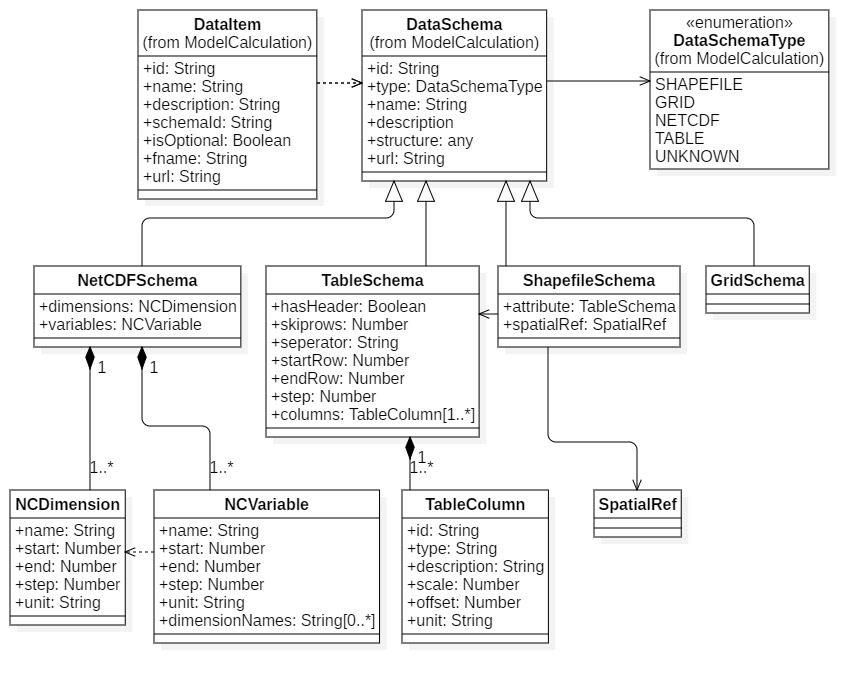
\includegraphics[width=.8\textwidth]{UML-data-description-interface}
    \caption{数据描述文档设计}
    \label{fig:UML-data-description-interface}
\end{figure}

为适应本文系统的架构,本文使用JSON Schema来具体地表达UDX Schema,使用原始数据格式作为UDX Data,这样既可以详尽地描述数据的元数据,又可以避免数据到XML的序列化和反序列化映射过程。

\subsubsection{NetCDF的UDX Schema模板}

\begin{figure}[!htbp]
    \centering
    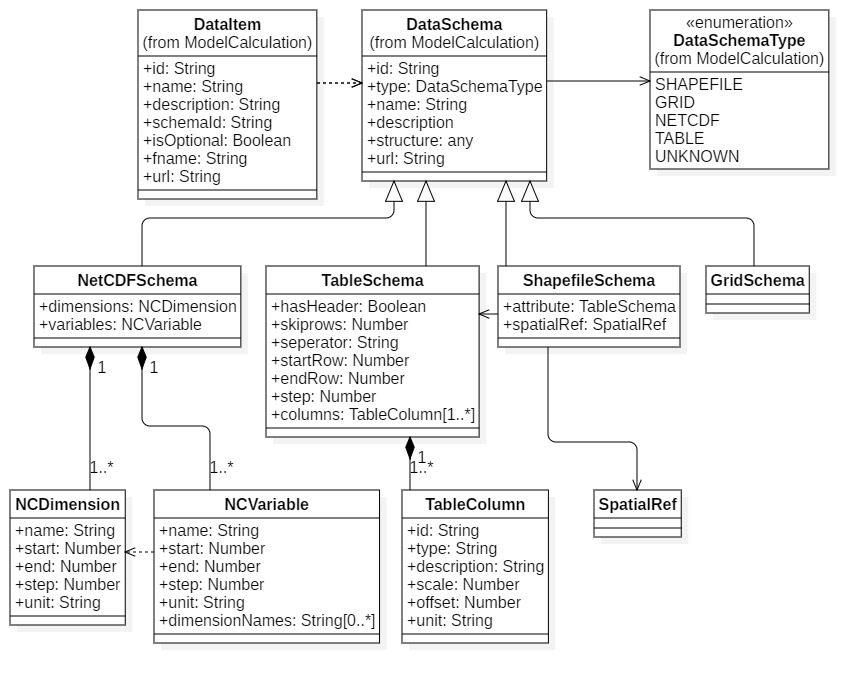
\includegraphics[width=.8\textwidth]{UML-data-description-interface}
    \caption{NetCDF描述文档}
    \label{fig:UML-data-description-interface}
\end{figure}

\subsubsection{CSV的UDX Schema模板}

\begin{figure}[!htbp]
    \centering
    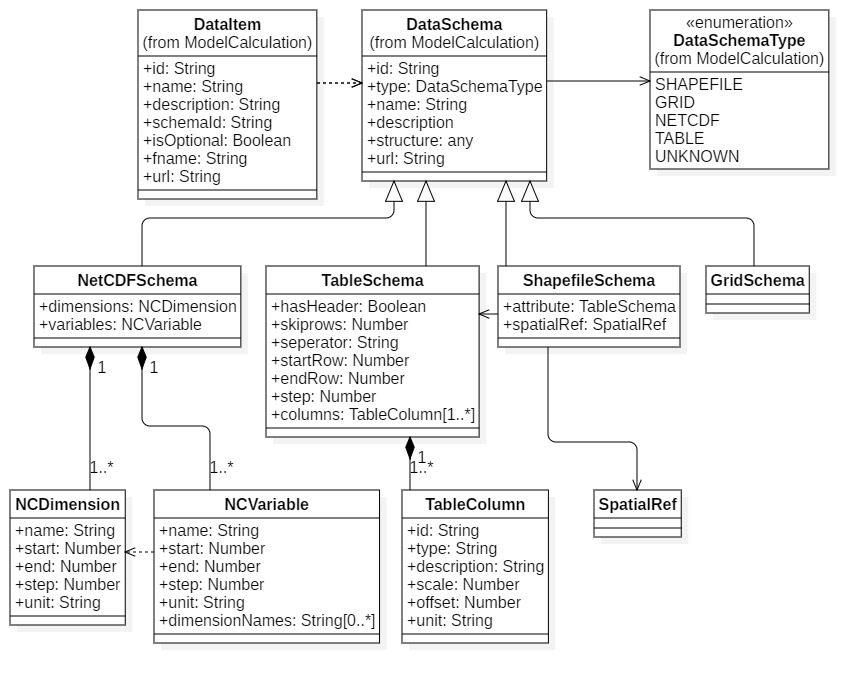
\includegraphics[width=.8\textwidth]{UML-data-description-interface}
    \caption{NetCDF描述文档}
    \label{fig:UML-data-description-interface}
\end{figure}

\subsubsection{Shapefile的UDX Schema模板}

\begin{figure}[!htbp]
    \centering
    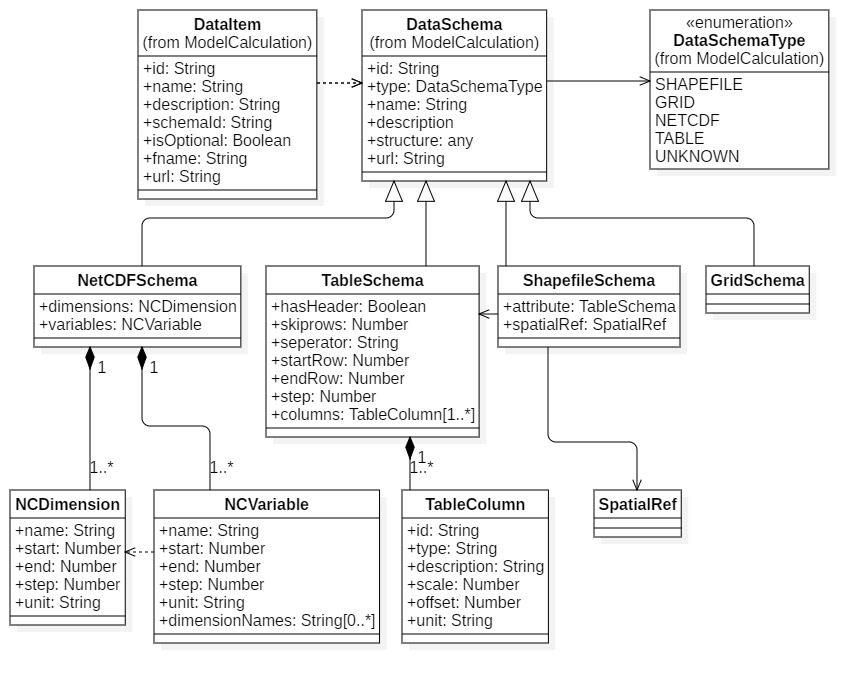
\includegraphics[width=.8\textwidth]{UML-data-description-interface}
    \caption{NetCDF描述文档}
    \label{fig:UML-data-description-interface}
\end{figure}

\subsection{碳循环相关数据资源的服务化封装}
\subsubsection{WMS/WFS/WCS}
\subsubsection{数据下载服务}
% 数据编排解析
\subsubsection{数据处理服务}
% schema 匹配

\section{开放式碳循环模型资源接入方法}
% 从支撑模型运行的角度出发,并结合地理模型对比的需求,梳理了地理模型的运行特征,并以结构化的文档描述模型资源,

\begin{figure}[!htbp]
    \centering
    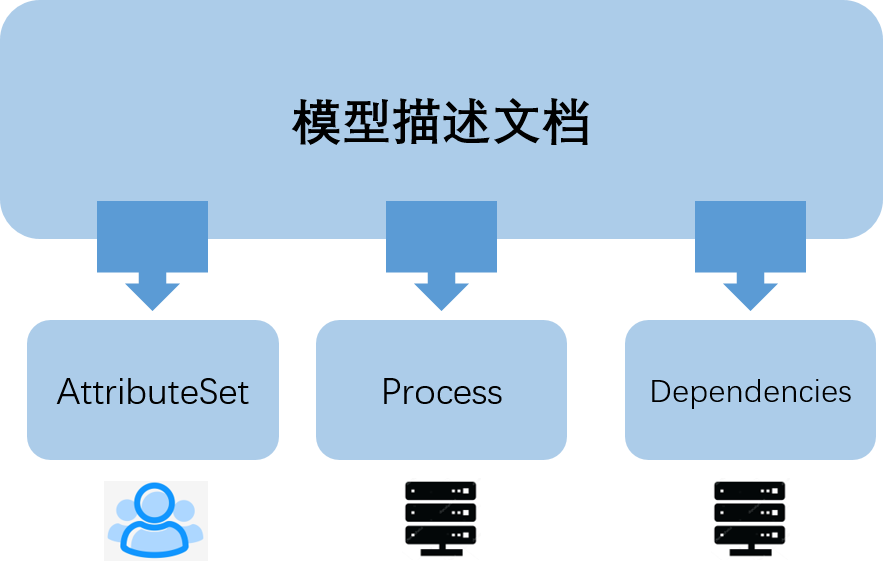
\includegraphics[width=1\textwidth]{mdl}
    \caption{模型服务的封装、发布和应用}
    \label{fig:mdl}
\end{figure}

\subsection{碳循环模型资源特征分析}
% 运行分类:简单型、时间推进型、条件语句型、多子过程的集成
% 运行进度
\begin{enumerate}[(1)]
    \item \textbf{模型参数策略特征}
    
    生态过程模型普遍采用植被功能类型(PFT)作为植被基本处理单元,通常将PFT划分为林地(覆盖热带、温带、寒带,常绿、落叶、针叶和阔叶等)、灌木(常绿和落叶等)、草地($C_3$、$C_4$等)、农田(水稻、玉米、温带谷物、大豆、热带根系作物、太阳花、花生、油菜等)等类型。每种植被功能类型对应有许多植被生理生态参数。

    \item \textbf{模型异构性分析}
    

\end{enumerate}

% 运行平台、语言、编译型解释型、有无源代码


\subsection{碳循环模型资源描述方法}
模型服务的描述方法是模型服务化的基础,其难点在于对于模型依赖数据的结构的有效表达和对于运行接口的标准化设计。模型服务描述文档应该是面向人的,通过模型服务描述文档提供的信息,模型服务使用者就能够方便地了解和使用模型,并能够理解模型的返回结果;同时模型服务描述文档又是面向机器的,通过模型服务描述文档提供的模型运行输入输出选项,能够判断出模型运行数据的完备性,并在用户发送请求时将模型调用起来。因此,本文将模型服务的描述文档设计为如图~\ref{fig:mdl}所示,
其中AttributeSet表示基本信息描述接口,面向人的理解;Beheavior表示模型的运行行为接口,面向机器理解模型的运行要求;Runtime表示模型的软硬件环境依赖,也是面向机器,支持模型能够成功调用起来。

模型描述文档由JSON形式表达,与本文选择的具体技术体系有关:一方面它与MongoDB数据库结构同构,有助于增删查改,另一方面它与后台服务器Node.js天生兼容,解析起来方便。

\begin{figure}[!htbp]
    \centering
    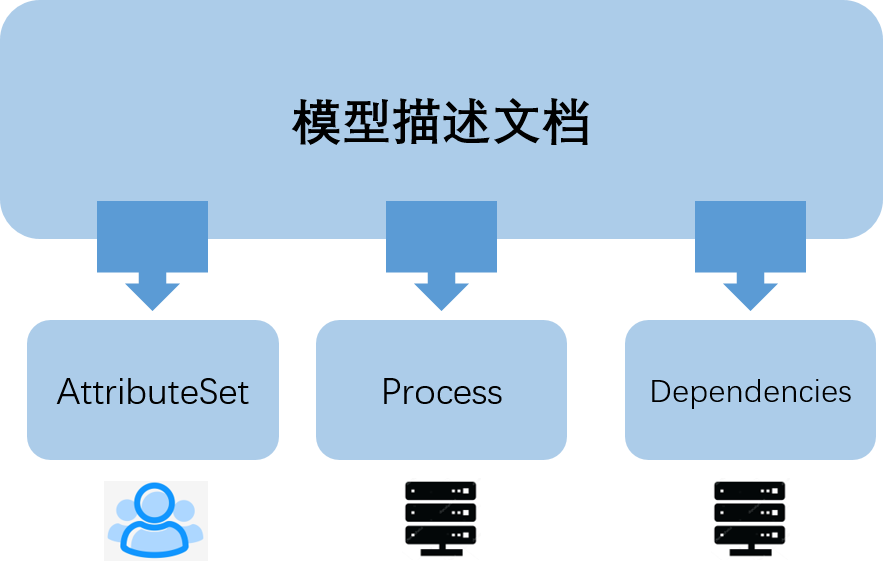
\includegraphics[width=1\textwidth]{mdl}
    \caption{模型描述文档设计}
    \label{fig:mdl}
\end{figure}

\subsubsection{基本信息描述接口设计}
% 名称、分类、作者、版本、
% 面向人和及其理解
基本信息
模型的基本信息包括模型名称、关键字、DOI、摘要、版本信息,并添加了wiki字段,使用markdown以可扩展的方式允许模型拥有者编辑。

\begin{figure}[!htbp]
    \centering
    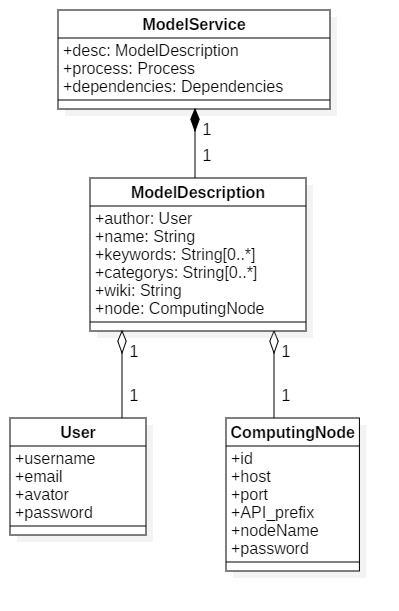
\includegraphics[width=.8\textwidth]{UML-model-description-interface}
    \caption{基本信息描述接口设计}
    \label{fig:UML-model-description-interface}
\end{figure}

\subsubsection{运行信息描述接口设计}
% 存储路径、文件名、类型(编译、解释)、
% 两个粒度:单模型运行和多模型集成
运行信息接口包括两部分:模型的输入输出列表和数据的格式

\begin{figure}[!htbp]
    \centering
    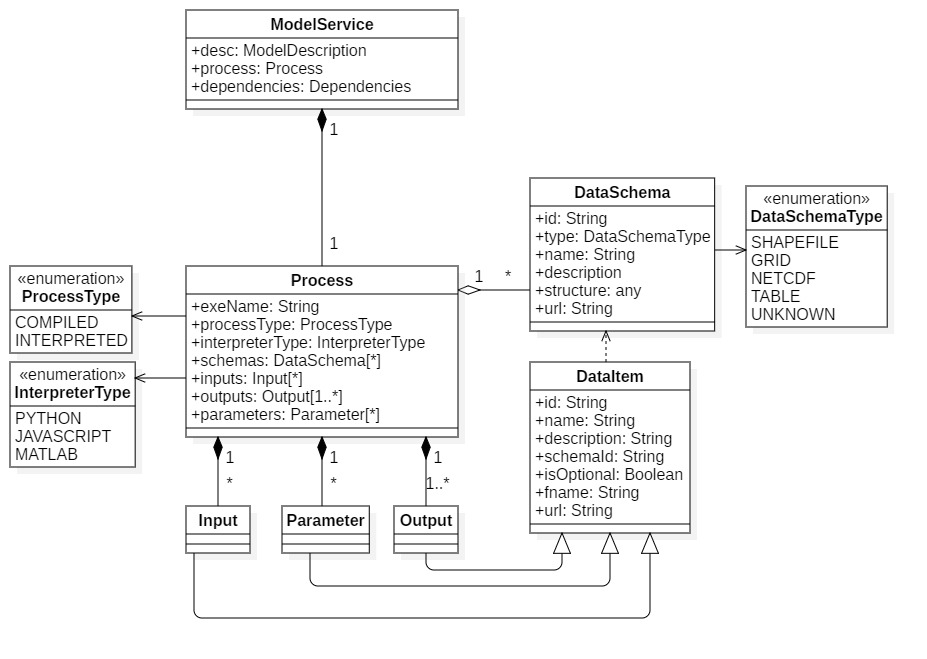
\includegraphics[width=1\textwidth]{UML-model-invoke-interface}
    \caption{运行信息描述接口设计}
    \label{fig:UML-model-invoke-interface}
\end{figure}

\subsubsection{部署信息描述接口设计}
% 软硬件依赖

\begin{figure}[!htbp]
    \centering
    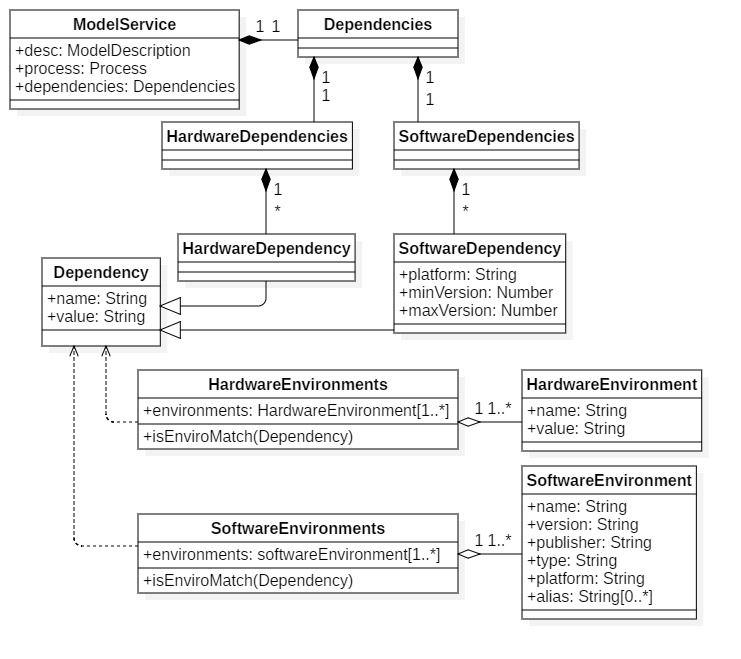
\includegraphics[width=1\textwidth]{UML-model-deployment-interface}
    \caption{部署信息描述接口设计}
    \label{fig:UML-model-deployment-interface}
\end{figure}

\subsection{碳循环模型资源的封装和服务发布}
\subsubsection{模型运行接口设计}
% 解释型、编译型

\subsubsection{服务封装}
% 几种方式:模型代理、源码封装

\subsubsection{服务部署和发布}
% 数据库录入条目、服务部署


\section{开放式碳循环模型对比方法}

\subsection{碳循环模型对比方法总结与归纳}
\subsubsection{统计学对比方法}
\textbf{加权超级集合}

\subsubsection{可视化对比方法}
\textbf{泰勒图}

\textbf{时间序列折线图}

\textbf{箱图}

\textbf{热力图}

\textbf{偏差等值线图}

\subsection{开放式碳循环模型对比方法接入方法}

\section{本章小结}
